%
%
%
%

\documentclass{article}
         
\usepackage{graphicx,xcolor}
\usepackage[load-headings]{exsheets}
\usepackage{bbding, skull}
\usepackage[frenchb]{babel}
\usepackage{amsmath,amssymb,bm}
\usepackage{enumitem}
\usepackage{lmodern,microtype}
\usepackage[a4paper,left=4cm,right=4cm]{geometry}
\usepackage{tikz}
\usepackage{hyperref}


\usetikzlibrary{arrows,decorations,calc}
\usetikzlibrary{decorations.pathmorphing,patterns,decorations.pathreplacing,decorations.markings}

\usepgflibrary{arrows}

\tikzset{
  % style to apply some styles to each segment of a path
  on each segment/.style={
    decorate,
    decoration={
      show path construction,
      moveto code={},
      lineto code={
        \path [#1]
        (\tikzinputsegmentfirst) -- (\tikzinputsegmentlast);
      },
      curveto code={
        \path [#1] (\tikzinputsegmentfirst)
        .. controls
        (\tikzinputsegmentsupporta) and (\tikzinputsegmentsupportb)
        ..
        (\tikzinputsegmentlast);
      },
      closepath code={
        \path [#1]
        (\tikzinputsegmentfirst) -- (\tikzinputsegmentlast);
      },
    },
  },
  % style to add an arrow in the middle of a path
  mid arrow/.style={postaction={decorate,decoration={
        markings,
        mark=at position .55 with {\arrow[#1]{stealth}}
      }}},
}



\renewcommand{\i}{\mathrm{i}}
\newcommand{\diff}{\text{d}}



\begin{document}
\noindent
{\textsc{Universit\'e catholique de Louvain}} \hfill \'Ecole de Physique\\
Facult\'e des Sciences \hfill 14 November 2024\\
\hrule

\bigskip

\begin{center}
  \textbf{Tutorial 5 -- Systems in three dimensions. Poincar\'e L'application de Poincar\'e} 
\end{center}

%\bigskip
\SetupExSheets{headings=runin-fixed-nr}


\subsection*{Three dimensional systems}

\begin{question} \textbf{Rikitake model.} The Rikitake equations are given by
  \begin{equation}
    \dot x = -\nu x + yz,\quad \dot y = -\nu y +(z-a)x, \quad \dot z = 1-xy,
  \end{equation}
where $a,\nu>0$ are parameters. These equations were proposed in 1958 as a model for the generation of the earth's magnetic field by the currents in the mantle.

\begin{enumerate}[label=(\alph*)]
  \item Show that the system is dissipative, meaning that volumes degrease over time.
  \item Show that the equilibriums are $(\pm k, \pm k^{-1},\nu k^2)$ where $k$ is a solution of $\nu(k^2-k^{-2})=a$. Classify these equilibria.
\end{enumerate}

Numerical simulations show that the model exhibits chaotic behaviour for certain parameter values. This behaviour is similar to the irregular reversals in the earth's magnetic field. A solution of the model is shown in Figure \ref{fig:Rikitake}.
\begin{figure}[h]
  \centering
    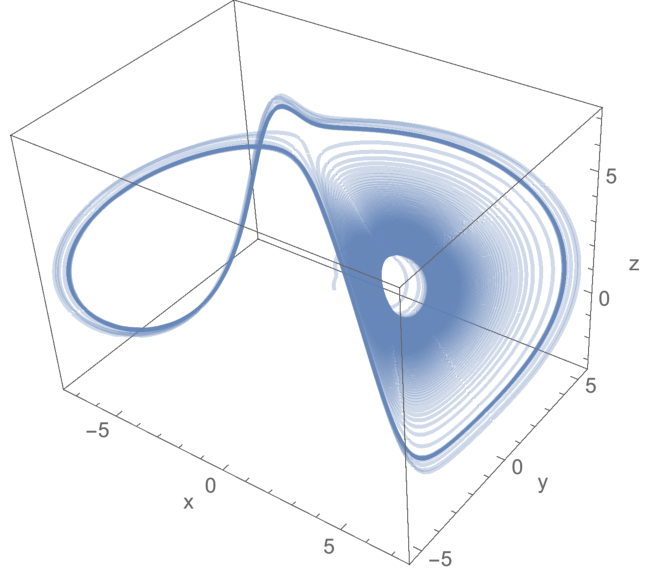
\includegraphics[scale=.8]{Rikitake}
    \caption{Orbit of a solution of the Rikitake model with $a=2,\nu=1/6$ and and initial condition $(x_0,y_0,z_0)=(0,1,0)$.}
  \label{fig:Rikitake}
\end{figure}

\end{question}

\begin{question} \textbf{Lorenz System for Large Reynolds Numbers.} We will investigate the Lorenz system in the limit $r\to \infty$. By taking this limit in a particular way we can make the dissipative terms disappear.

\begin{enumerate}[label=(\alph*)]
  \item We will let $\epsilon = r^{-1/2}$. In the limit $r\to \infty$ we have $\epsilon \to 0$. Find a change of variables $x,y,z,t\to X,Y,Z,\tau$ dependant on $\epsilon$ as $\epsilon \to 0$ the lorenz system becomes:
  \begin{equation}
    \dot X = Y, \quad \dot Y = - XZ, \quad \dot Z= XY.
  \end{equation}
  \item Show that the new system is not dissipative: That it conserves volumes over time.
  \item Find two conserved quantities for the new system (these are $E=E(X,Y,Z)$ where $\dot E=0$.) Discuss the consequences of the existence of the existence of these conserved quantities.
\end{enumerate}
\end{question} 


\subsection*{Poincar\'e Sections}
\begin{question} \textbf{Logistic equation with a periodic forcing.} In this exercise we consider a model for the evolution of a population. The equation is given by $\dot x = f(t,x)$ with
\begin{equation}
  f(t,x) = a x(1-x) -h(1+\sin 2\pi t)
\end{equation}
where $a,h>0$ are constants. The first term corresponds to growth rate given by the logistic equation. The second term represents a diminishing term of the population which varies with time $t$.

\begin{enumerate}[label=(\alph*)]
  \item Show that if $x(t)$ is a solution of the differential equation then $x(t+1)$ is also a solution. Show that it is sufficient to constrain the solutions between $0 \leqslant t \leqslant 1$.
  \item Given $\phi(t,x_0) = \phi^t(x_0)$ is a unique solution with the initial condition $x_0$ at $t=0$. We define a \textit{Poincar\'e section} by $p(x_0) = \phi(t=1,x_0)$. Show that if $x_0$ is a fixed point, i.e. $p(x_0) = x_0$ then the solution is a periodic solution of period $T=1$.
  \item Show that
  \begin{equation}
    \label{eqn:KeyRelation}
    \frac{\partial \phi(t,x_0)}{\partial x_0} = \exp\left(\int_0^t f_x(s,\phi(s,x_0))\diff s\right)
  \end{equation}
  where $f_x(t,x) = \partial f(t,x)/\partial x$ is a partial derivative of $f$ with respect to $x$. Show that $p'(x_0)>0$.
  \item By differentiating \eqref{eqn:KeyRelation} with respect to $x_0$, and show that $p''(x_0) < 0$. Show that the Poincar\'e section has at least two fixed points. \textit{Hint: } It is useful to make $p(x_0)$ as a function of $x_0$.
  \item Show that $p(x_0)$ is dependant on the value of $h$. Deduce that there exists a unique value $h=h_c$ where this Poincar\'e section that has exactly one fixed point. For $h>h_c$, no fixed point exists. What is the significance for the evolution of the population?
\end{enumerate}
The behaviour of the solutions for $h<h_c$ is shown in Figure \ref{fig:LogisticPeriodic}. 

\begin{figure}[h]
  \centering
  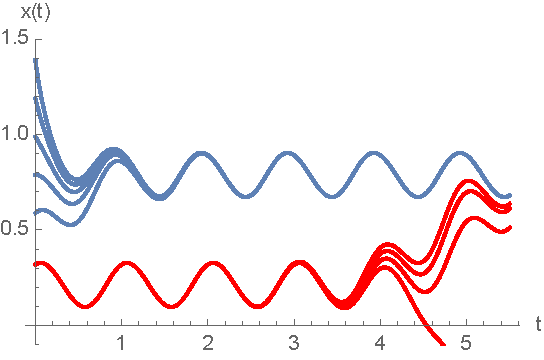
\includegraphics[scale=.8]{PeriodicSolutions}
  \caption{The different types of solutions for $a=5,\,h=0.8<h_c$. The Poincar\'e section has two fixed points $x_0^+= 0.78865731\dots$ et $x_0^-= 0.31866561\dots$, corresponding two periodic solutions. For sufficiently large $x(t=0)=x_0$ the solutions converge towards the periodic solutions corresponding to $x_0^+$. The solutions with $x_0$ close to $x_0^-$ diverges from the periodic solution.}
  \label{fig:LogisticPeriodic}
\end{figure}

\end{question}
\end{document}

